\documentclass[a4paper]{article}

%use the english line for english reports
%usepackage[english]{babel}
\usepackage[portuguese]{babel}
\usepackage[utf8]{inputenc}
\usepackage{indentfirst}
\usepackage{graphicx}
\usepackage{subfig}
\usepackage{verbatim}
\usepackage{listings} 


\begin{document}

\setlength{\textwidth}{16cm}
\setlength{\textheight}{22cm}

\title{\Huge\textbf{MOD X}\linebreak\linebreak\linebreak
\Large\textbf{Relatório Intercalar}\linebreak\linebreak
\linebreak\linebreak

\includegraphics[scale=0.1]{./images/feup-logo.png}\linebreak\linebreak
\linebreak\linebreak
\Large{Mestrado Integrado em Engenharia Informática e Computação} \linebreak\linebreak
\Large{Programação em Lógica}\linebreak
}

\author{\textbf{Grupo ModX3:}\\
António Manuel Vieira Ramadas - 201303568 \\
Rui Miguel Teixeira Vilares - 201207046 \\
\linebreak\linebreak \\
 \\ Faculdade de Engenharia da Universidade do Porto \\ Rua Roberto Frias, s\/n, 4200-465 Porto, Portugal \linebreak\linebreak\linebreak
\linebreak\linebreak\vspace{1cm}}

\maketitle
\thispagestyle{empty}

%************************************************************************************************
%************************************************************************************************

\newpage

%Todas as figuras devem ser referidas no texto. %\ref{fig:codigoFigura}
%
%%Exemplo de código para inserção de figuras
%%\begin{figure}[h!]
%%\begin{center}
%%escolher entre uma das seguintes três linhas:
%%\includegraphics[height=20cm,width=15cm]{path relativo da imagem}
%%\includegraphics[scale=0.5]{path relativo da imagem}
%%\includegraphics{path relativo da imagem}
%%\caption{legenda da figura}
%%\label{fig:codigoFigura}
%%\end{center}
%%\end{figure}
%
%
%\textit{Para escrever em itálico}
%\textbf{Para escrever em negrito}
%Para escrever em letra normal
%``Para escrever texto entre aspas''
%
%Para fazer parágrafo, deixar uma linha em branco.
%
%Como fazer bullet points:
%\begin{itemize}
	%\item Item1
	%\item Item2
%\end{itemize}
%
%Como enumerar itens:
%\begin{enumerate}
	%\item Item 1
	%\item Item 2
%\end{enumerate}
%
%\begin{quote}``Isto é uma citação''\end{quote}


%%%%%%%%%%%%%%%%%%%%%%%%%%
\section{O Jogo MOD X}

\subsection{Contextualização}
O MOD X é um jogo de tabuleiro, nascido em 2015, recomendado para jogadores com mais de 15 anos de idade.
É um jogo de estratégia, divertido e fácil de aprender.
Cada partida reúne 2 a 4 jogadores e tem a duração prevista de 20 a 30 minutos. 

\subsection{Componentes do jogo}
\begin{itemize}
	\item 1 Tabuleiro 8x8;
	\item 56 peças de jogo em formato X (14 em cada cor);
	\item 72 marcadores de pontuação (18 em cada cor);
	\item 5 peças \textit{Joker} em formato X (brancas);
\end{itemize}

\begin{figure}[h!]
	\begin{center}
		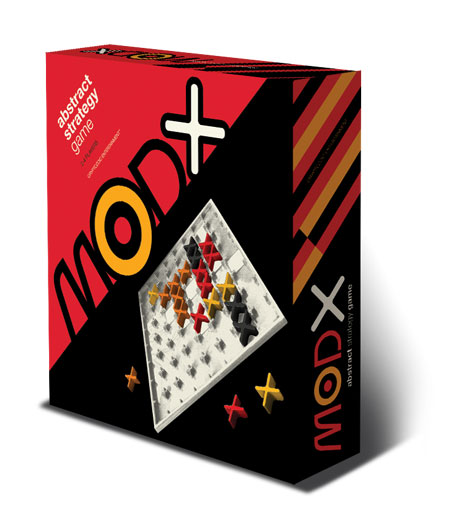
\includegraphics[scale=0.3]{./images/modx_box.jpg}
		\caption{Caixa do MOD X}
		\label{fig:1}
	\end{center}
\end{figure}

\subsection{Objetivo do jogo}

O objetivo deste jogo é criar padrões com peças coloridas (vermelho, preto, amarelo e laranja).
Pretende-se assim, formar o maior número de padrões possível, de forma a conseguir a melhor pontuação.
O vencedor é o jogador com mais pontos.
Evidentemente, é também suposto bloquear os adversários de modo que não consigam construir esses padrões\footnote{https://boardgamegeek.com/boardgame/131387/mod-x}.  

\subsection{Regras}

\begin{itemize}
	\item Define-se a ordem dos jogadores, cada um escolhe a cor das suas peças e define-se o limite de pontos\footnote{https://www.cryptozoic.com/games/mod-x};
	\item Cada jogador inicia o jogo com 14 peças e 18 marcadores;
	\item Os \textit{Jokers} são dispostos inicialmente de forma aleatória no tabuleiro; 
	\item No seu turno, cada jogador coloca uma peça no tabuleiro, em qualquer posição livre;
	\item Os padrões utilizados para ganhar pontos são o ''X'', o ''+'' e o ''cinco em linha'';
	
	\begin{figure}[h!]
		\begin{center}
			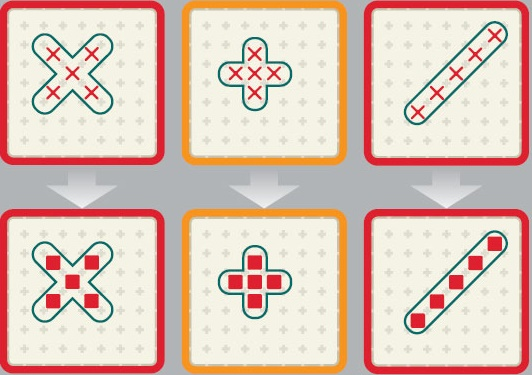
\includegraphics[scale=0.4]{./images/modx_score.jpg}
			\caption{Padrões usados}
			\label{fig:2}
		\end{center}
	\end{figure}
	
	\item O jogador pode usar os \textit{Jokers} para formar padrões, como se das suas próprias peças se tratassem;
	\item Quando um padrão é formado, retiram-se as peças de jogo e introduzem-se marcadores nessas posições. As peças de jogo podem agora voltar a ser utilizadas e as casas com marcadores também;
	\item Cada marcador colocado corresponde a um ponto.
	\item Caso tenha sido usado um \textit{Joker} para formar um padrão, nessa posição não é introduzido um marcador. O \textit{Joker} é agora colocado numa posição ao critério do jogador. Atenção, o \textit{Joker} não pode ser usado para formar um novo padrão de imediato; 
	
	\begin{figure}[!h]
		\centering
		\subfloat[Peças]{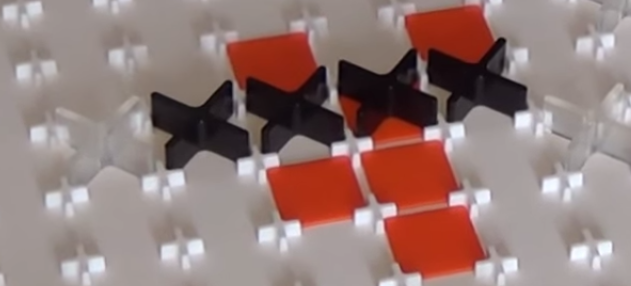
\includegraphics[width=0.3\textwidth]{./images/padroesPretos.png}\label{fig:f1}}
		\hfill
		\subfloat[Marcadores]{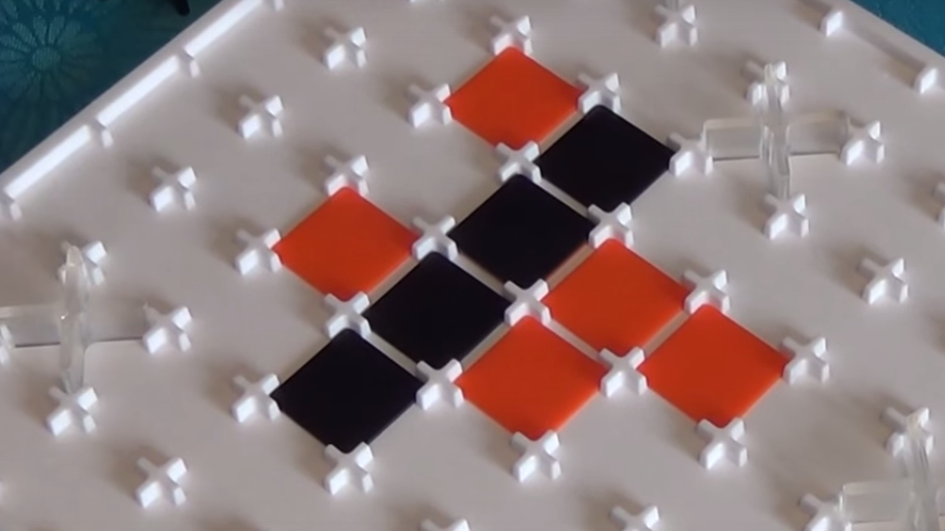
\includegraphics[width=0.3\textwidth]{./images/padroesPretosMarcadores.png}\label{fig:f2}}
		\caption{Substituição das peças por marcadores}
	\end{figure}
	
	\item O primeiro jogador a atingir o número de pontos, determinado inicialmente, é o vencedor.
	\item O jogo pode também acabar quando um jogador já não dispõe de peças ou marcadores. Nesse caso, ganha o jogador com mais pontos até ao momento. 
	

	
\end{itemize}
%%Cada jogador inicia o jogo com 14 peças e 18 marcadores.
%%Inicialmente, define-se a ordem dos jogadores e escolha das peças por parte dos jogadores.  
%%No seu turno, um jogador coloca uma peça no tabuleiro, com o objetivo de criar padrões específicos, que se traduzem em pontos.
%%Os padrões utilizados para ganhar pontos são o ''X'', o ''+'' e o ''cinco em linha''.

%%Existem umas peças de cor branca, dispostas inicialmente de forma aleatória, chamadas Jokers. O jogador pode usar essas peças para formar padrões, como se tratassem das suas próprias peças.

%%É suposto bloquear os adversários de modo que não consigam construir esses padrões\footnote{https://www.cryptozoic.com/games/mod-x}.

%%No final, o primeiro jogador a atingir um certo número de pontos, determinado inicialmente pelo número de jogadores, é o vencedor.
%%O jogo pode também terminar quando um jogador terminar com as suas peças ou marcadores.
%%Nesse caso, o jogo termina imediatamente e ganha o jogador com mais pontos até ao momento.


%%%%%%%%%%%%%%%%%%%%%%%%%%
\section{Representação do Estado do Jogo}

\subsection{Representação do estado inicial do tabuleiro}

%%printBoard(
\begin{small}
\begin{lstlisting}
[[-1,-1],[-1,-1],[-1,-1],[-1,-1],[-1,-1],[-1,-1],[-1,-1],[-1,-1],
[-1,-1],[0,-1],[1,-1],[2,-1],[2,-1],[1,-1],[0,-1],[-1,-1],
[-1,11],[0,11],[1,11],[2,11],[2,11],[1,11],[0,11],[-1,11],
[-1,22],[0,22],[1,22],[2,22],[2,22],[1,22],[0,22],[-1,22],
[-1,-1],[0,-1],[1,-1],[2,-1],[2,-1],[1,-1],[0,-1],[-1,-1],
[-1,11],[0,11],[1,11],[2,11],[2,11],[1,11],[0,11],[-1,11],
[-1,22],[0,22],[1,22],[2,22],[2,22],[1,22],[0,22],[-1,22],
[-1,-1],[-1,-1],[-1,-1],[-1,-1],[-1,-1],[-1,-1],[-1,-1],[-1,-1]]
\end{lstlisting}
\end{small}
%%).

INSERIR IMAGEM


\subsection{Representação de um estado intermédio do tabuleiro}

INSERIR CODIGO

INSERIR IMAGEM

\subsection{Representação de um estado final do tabuleiro}

INSERIR CODIGO

INSERIR IMAGEM

%%%%%%%%%%%%%%%%%%%%%%%%%%
\section{Visualização do Tabuleiro}




%%%%%%%%%%%%%%%%%%%%%%%%%%
\section{Movimentos}

\textbf{Falha se o \textit{Joker} é posto numa posição errada}\newline
\begin{small}
placeJoker(Board, Player, TileNumber).
\end{small}\newline

\textbf{Devolve as jogadas possíveis em ListOfMoves}\newline
\begin{small}
validMoves(Board, Player, ListOfMoves).
\end{small}\newline

\textbf{Falha se não poder ser feito o movimento}\newline
\begin{small}
move(Board, Player, TileNumber, NewBoard).
\end{small}\newline

\textbf{Avalia a jogada e devolve o seu valor em Value}\newline
\begin{small}
value(Board, Player, TileNumber, Value).
\end{small}\newline

\textbf{Caso o jogo tenha acabado devolve o vencedor em Winner}\newline
\begin{small}
gameOver(Board, Winner).
\end{small}\newline

\textbf{Jogada do computador em que consoante diferentes níveis de dificuldade (Level) devolve jogadas diferentes}\newline
\begin{small}
choose\_Move(Board, Level, Move).
\end{small}\newline

\textbf{Põe as bases e tira as cruzes do jogador Player}\newline
\begin{small}
putTiles(Board, Player, NewBoard).
\end{small}\newline


\end{document}
